\renewcommand\TheFile{gui.tex}
\SVN $Author: hom $
\SVN $Revision: 126 $
\SVN $Id: gui.tex 126 2017-10-24 07:34:14Z hom $
\SVN $Date: 2017-10-24 09:34:14 +0200 (di, 24 okt 2017) $
\SVN $State: Exp $
\begin{savequote}[8cm]
  \sffamily
  All our dreams can come true, if we have the courage to pursue them.
  \qauthor{Walt Disney}
\end{savequote}
\chapter{Graphical user interface}

\parpic(60mm,45mm)[rs]{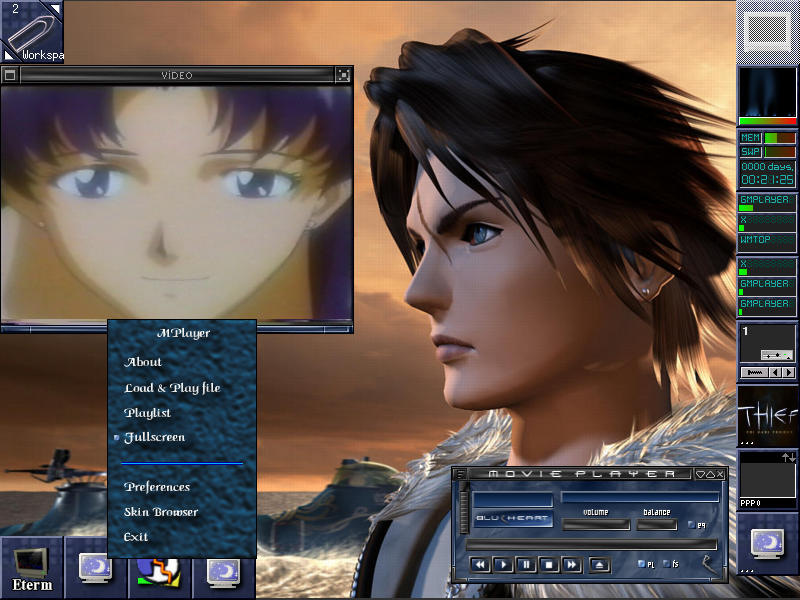
\includegraphics[width=58mm]{figures/gui-preview-02.jpg}}The current hardware model is somewhat limited and misses some
features that you would expect in a real elevator system.

To make the modelling more realistic we compensate for these missing
features in the graphical user interface.

You should use the JavaFX framework to implement the graphical
user interface of the system. There are a number of nice tutorials on
the web, such as \url{https://docs.oracle.com/javafx/2/get_started/jfxpub-get_started.htm}
at the Oracle website.

If you want to implement annimations, visit \url{https://docs.oracle.com/javafx/2/animations/basics.htm}.

The JFXtras at \url{http://jfxtras.org/} has some nice widgets that  might be handy in you implementation.
 
\section{GUI features}

\paragraph{Lit buttons} In a modern elevator system you expect lit
buttons. Once a button is pressed, the button is lit. This light
stays on until the service requested by the passenger is
provided. As an example: when a passenger presses an UP button on
floor f, the button's light stays on until a cage visits floor f in
an upward journey. In the GUI presentation all buttons should have
lights.

\paragraph{Obstruction detection} A modern elevator, or any
automatically closing door for that matter, will have some kind of an 
obstruction sensor. In the GUI this sensor can be simulated by
implementing the GUI cage as some kind of button, in which the pressed
state equals obstruction.

\paragraph{Door Open and close buttons} A cage in an elevator system should
have an open and a close button, that requests the door to be opened
or closed. Once an elevator has a request which takes it to another
floor, the door is closed. If a cage stops at a floor a transfer
timeout must be observed, which can be shortened by pressing the door
close button and extended by pressing the door open button. Of course
the door should only open if the cage is at rest at a floor.

\parpic(60mm,35mm)[r]{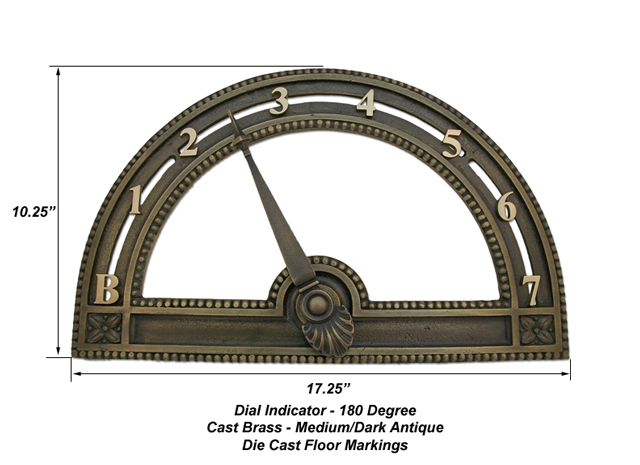
\includegraphics[width=58mm]{figures/180dialbrassnumbers.jpg}}\paragraph{Cage position indication} As in the hardware model, the GUI
should also show the whereabouts of the cage on some kind of indicator
on each floor. The same approach as the hardware (two lights when
between floors) can be used. A dial model, such as used in old
fashioned elevator systems would be a very nice touch.

\paragraph{Multiple cages} A serious elevator system would have multiple
cages, making a strategy for up and down buttons more meaningful to
system and passengers. In your implementation you should be able to
support at least two cages in the GUI, where one of these GUI cages
will monitor the hardware elevator model. The idea is that this GUI cage
presents the behaviour of the hardware model, synchronous to that
model. You should try to make an attempt to let the GUI and the
hardware model move as synchronously as possible. The GUI cage will
have all the missing features as mentioned above and otherwise mimic
the hardware model faithfully. For instance if the red button is used
as the obstruct button, and the monitor provides obstruction
behaviour, then both the hardware cage and this monitor cage should
reopen its door and wait for the obstruction to be removed.  

\paragraph{Nurse button} The nurse button should also be present in
the GUI.

\paragraph{Number of floors} The GUI design should be able to support
at least 10 floors. 

\paragraph{Logging} The system should log all up and down requests and
arrivals as well as the motor cycles of all cages. (Up, down, stop).
The tail of this log (the last entries) should be shown in the GUI.

\paragraph{Floor announcement} Once the elevator stops at a floor due
to a target request, an audible floor announcement is given. In an
extended version of the system, this floor announcement may
have a different announcement signal for each floor. Simple but
distinct sounds can be used but thinkable is something like
\textit{``fourth floor, 
  penthouse and restaurant''}. The floor announcement system could
also be used to inform the passengers of special situations like out
of order messages and the like.


